% ======================================================================
%  Chapter 16 — Synthetic Dimensions  (DEEPLY EXPANDED)
%  photonic systems, including Harper-Hofstadter, 4D QHE, experiments
\cite{kane2005sub}.
% ======================================================================

\section{Beyond physical dimensions}
\label{sec:ch16-intro}

The topological phenomena explored in Chapters~7--15 occur in systems
with two or three spatial dimensions.  But topology is not limited by
the number of physical dimensions: it depends on the structure of the
Hilbert space and the connectivity of the parameter manifold, not on the
spatial geometry of the laboratory.

A \emph{synthetic dimension} is an internal degree of freedom---such as
the frequency, orbital angular momentum, spin, or mode index of a
photon---that is reinterpreted as an extra spatial coordinate through
engineered couplings.  By coupling modes along the synthetic axis with
controlled phases, one can create effective lattice models in dimensions
higher than the physical space \cite{lin2018constructing}.  This opens a route to observing
topological phases that have no direct analog in lower-dimensional
systems, most notably the four-dimensional quantum Hall effect.

This chapter derives the synthetic-dimension framework from Maxwell's
equations \cite{ozawa2018topological,liu2021observation}, explains how the Harper--Hofstadter model and higher-dimensional
Chern insulators can be implemented in photonic systems, and surveys the
principal experimental platforms \cite{kim2020recent}.

\section{Frequency as a synthetic dimension}
\label{sec:ch16-frequency}

\subsection{The coupled-mode picture}
\label{sec:ch16-coupled-mode}

Consider a ring resonator supporting a comb of equally spaced resonant
frequencies $\omega_m=\omega_0+m\Omega_{\mathrm{FSR}}$
($m=0,\pm 1,\pm 2,\ldots$), where $\Omega_{\mathrm{FSR}}=2\pi c/(n_g L)$
is the free spectral range, $n_g$ is the group index, and $L$ is the
round-trip length
\cite{press2026photonic}.  In the absence of modulation, the modes are
decoupled and the frequency index $m$ labels a one-dimensional lattice
with lattice constant $\Omega_{\mathrm{FSR}}$.

Now apply an electro-optic phase modulation at frequency
$\Omega_{\mathrm{mod}}=\Omega_{\mathrm{FSR}}$ to the resonator.  The
modulation creates a time-dependent coupling between adjacent frequency
modes.  In the slowly varying envelope approximation, the amplitude
$a_m(t)$ of mode $m$ satisfies the coupled-mode equation
\begin{equation}\label{eq:ch16-coupled-mode}
  \ii\pderiv{a_m}{t}
  = \omega_m\,a_m + \kappa\bigl(\ee^{\ii\phi}\,a_{m-1}
  + \ee^{-\ii\phi}\,a_{m+1}\bigr)\,,
\end{equation}
where $\kappa$ is the modulation strength and $\phi$ is the modulation
phase.  This is mathematically identical to the tight-binding equation
for a particle hopping on a 1D lattice with nearest-neighbour coupling
$\kappa\ee^{\pm\ii\phi}$.

The frequency axis has thus become a \emph{synthetic spatial dimension}:
hopping along the frequency ladder is controlled by the electro-optic
modulation, and the hopping phase $\phi$ plays the role of a Peierls
phase (synthetic gauge field)
\cite{raghu2008analogs}.

\begin{figure}[t]
  \centering
  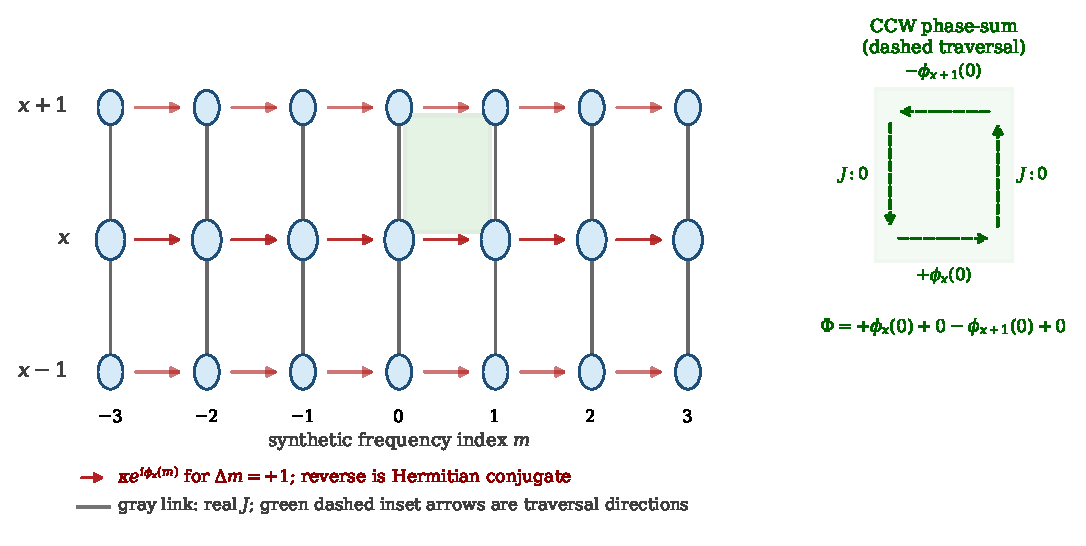
\includegraphics[width=0.88\textwidth]{figures/fig_synthetic_frequency_ladder.pdf}
  \caption{Synthetic frequency dimension in a modulated resonator
    array.  Each column represents a frequency mode
    $\omega_m=\omega_0+m\Omega$; each row represents a physical
    resonator at real-space site $x$.  Red rightward arrows denote
    the Peierls hopping $\kappa\ee^{\ii\phi_x(m)}$ along the
    synthetic frequency direction ($\Delta m=+1$); the reverse
    ($\Delta m=-1$) hopping is the Hermitian conjugate \cite{yuan2018synthetic,yuan2015photonic}.  Gray
    vertical links represent the real-valued inter-site coupling $J$.
    The green shaded plaquette between columns $m=0$ and $m=1$ at
    sites $x$ and $x{+}1$ carries a gauge-invariant flux
    $\Phi=\phi_x(0)-\phi_{x+1}(0)$, computed by summing the
    directed link phases counter-clockwise.  In the inset this is
    displayed as $+\phi_x(0)+0-\phi_{x+1}(0)+0$: the two vertical
    $J$ links contribute zero phase.  In the inset, the dashed green
    arrows show the traversal directions used for this phase sum,
    whereas the red arrows in the main lattice show the physical
    hopping direction $\Delta m=+1$.  This flux is the
    synthetic-dimension analog of an applied magnetic field.}
  \label{fig:ch16-synthetic-ladder}
\end{figure}

\subsection{Derivation from Maxwell's equations}
\label{sec:ch16-maxwell-derivation}

To maintain the Maxwell-first spirit of this book, we derive the
coupled-mode equation \eqref{eq:ch16-coupled-mode} from the
time-dependent Maxwell equations with a modulated material matrix.

Consider a ring resonator whose permittivity is modulated:
\begin{equation}\label{eq:ch16-eps-modulated}
  \varepsilon(t) = \bar\varepsilon\bigl[1 + 2\eta\cos(\Omega_{\mathrm{mod}}t-\phi)\bigr] \,.
\end{equation}
Here $\eta\ll 1$ is the modulation depth.  The minus sign in
\eqref{eq:ch16-eps-modulated} is a convention: with fields written as
$\ee^{-\ii\omega t}$, it makes $\phi$ the Peierls phase for the
rightward frequency transition $m\to m+1$.  If the physical drive is
instead written as $\cos(\Omega_{\mathrm{mod}}t+\theta)$, then the
Peierls phase used below is $\phi=-\theta$.  The electric field in the
resonator is expanded in the unperturbed mode basis:
$E(t)=\sum_m a_m(t)\,\mathcal E_m\,\ee^{-\ii\omega_m t}$, where
$\mathcal E_m$ is the mode profile of mode $m$.

Substituting into the Maxwell wave equation and using the rotating-wave
approximation (retaining only the slowly varying terms), one obtains
\begin{equation}\label{eq:ch16-rwa}
  \ii\dot{a}_m = \kappa_{\mathrm{eff}}\bigl(\ee^{\ii\phi}\,a_{m-1}
  + \ee^{-\ii\phi}\,a_{m+1}\bigr)\,,
\end{equation}
The phase factors in \eqref{eq:ch16-rwa} follow directly from the
time convention just fixed: the coupling from $m-1$ to $m$ uses the
$\ee^{-\ii\Omega_{\mathrm{mod}}t+\ii\phi}$ component of the modulation,
whereas the coupling from $m+1$ to $m$ uses the complex-conjugate
component.  Thus the rightward hopping carries $+\phi$ and the reverse
hopping carries $-\phi$, matching \figref{fig:ch16-synthetic-ladder}.
The effective coupling is
\begin{equation}\label{eq:ch16-coupling}
  \kappa_{\mathrm{eff}} = \frac{\eta\omega_0}{2}
  \frac{\int|\mathcal E_m|^2\varepsilon_0\,\dd V}
  {\int|\mathcal E_m|^2\bar\varepsilon\,\dd V}
  \approx \frac{\eta\omega_0}{2}\,.
\end{equation}
This confirms that the coupled-mode equation
\eqref{eq:ch16-coupled-mode} is a direct consequence of the Maxwell
equations with a time-modulated permittivity.

\section{The Harper--Hofstadter model from synthetic dimensions}
\label{sec:ch16-harper}

\subsection{Adding a physical dimension}
\label{sec:ch16-2d-lattice}

To create a 2D lattice, we combine the synthetic frequency dimension
with one physical spatial dimension.  Consider an array of $N$ coupled
ring resonators, each supporting a frequency comb and each individually
modulated.  The physical coupling between adjacent rings provides
hopping along the spatial direction $x$, and the intra-ring modulation
provides hopping along the synthetic frequency direction $m$.

The amplitude $a_{m,x}(t)$ of mode $m$ in ring $x$ satisfies
\begin{equation}\label{eq:ch16-2d-hamiltonian}
  \ii\dot{a}_{m,x}
  = J\bigl(a_{m,x-1}+a_{m,x+1}\bigr)
  + \kappa\bigl(\ee^{\ii\phi_x}a_{m-1,x}+\ee^{-\ii\phi_x}a_{m+1,x}\bigr)\,,
\end{equation}
where $J$ is the inter-ring coupling and $\phi_x=\phi_0+\alpha x$ is
the modulation phase that varies linearly along the array.

\subsection{Mapping to the Hofstadter Hamiltonian}
\label{sec:ch16-hofstadter}

In the Bloch-wave ansatz $a_{m,x}=\ee^{\ii(k_x x + k_m m)}b_{m,x}$,
the equation of motion \eqref{eq:ch16-2d-hamiltonian} becomes
\cite{ozawa2018topological}
\begin{equation}\label{eq:ch16-hofstadter}
  \boxed{%
  E\,b_{m,x} = 2J\cos(k_x)\,b_{m,x}
  + 2\kappa\cos(k_m+\alpha x+\phi_0)\,b_{m,x}\,,}
\end{equation}
which is the \emph{Harper equation}, the eigenvalue equation of the
Hofstadter model with flux $\alpha$ per plaquette.  When
$\alpha/(2\pi)=p/q$ is a rational number, the spectrum splits into $q$
subbands, forming the famous Hofstadter butterfly.

The key insight is that the synthetic gauge flux $\alpha$ is fully
controllable through the modulation phase gradient.  By choosing
$\alpha=2\pi p/q$ for small $q$, one can access topological regimes
(nonzero Chern numbers) with experimentally reasonable modulation
parameters.

\subsection{Topological bands and edge states}
\label{sec:ch16-harper-topology}

Each subband of the Harper equation carries a Chern number determined by
the Diophantine equation $\Chern_r = \sigma_r$, where $\sigma_r$ is
the quantised Hall conductance of the $r$-th gap.  For
$\alpha/(2\pi)=1/3$ (three subbands), the Chern numbers are
$\Chern_1=+1$, $\Chern_2=-2$, $\Chern_3=+1$.

In the synthetic-dimension realisation, the ``edge'' of the frequency
lattice is set by the finite bandwidth of the modulation or the gain
medium.  Edge states appear at the boundary of the synthetic lattice
and propagate unidirectionally along the physical direction, directly
analogous to quantum Hall edge states.

\section{Four-dimensional quantum Hall effect}
\label{sec:ch16-4d}

\subsection{Topology in four dimensions}
\label{sec:ch16-4d-topology}

In four spatial dimensions, the quantum Hall effect is characterised by
the \emph{second Chern number}, a topological invariant defined on the
4D Brillouin zone $T^4$:
\begin{equation}\label{eq:ch16-second-chern}
  \Chern_2 = \frac{1}{8\pi^2}\int_{T^4}
  \Tr(\mathcal{F}\wedge\mathcal{F})\,,
\end{equation}
where $\mathcal{F}$ is the non-Abelian Berry curvature 2-form of the
occupied bands (Appendix~B).  The 4D quantum Hall effect predicts a
\emph{nonlinear} Hall response: a current perpendicular to three
applied fields, with a quantised coefficient proportional to $\Chern_2$.

The second Chern number is fundamentally different from the first Chern
number: it requires at least four dimensions to be nonzero and detects
topological features (``instanton-like'' structures in the Berry
connection) that have no analog in lower dimensions.

\subsection{Synthetic 4D lattice}
\label{sec:ch16-4d-lattice}

To realise a 4D topological system in a photonic experiment, one
combines two physical dimensions with two synthetic dimensions.  For
example, a 2D array of ring resonators, each modulated at two
frequencies $\Omega_1$ and $\Omega_2$, creates a 4D lattice with
coordinates $(x,y,m_1,m_2)$, where $x,y$ are physical positions and
$m_1,m_2$ are frequency-mode indices along the two synthetic axes.

The effective 4D Hamiltonian can be engineered to have nonzero $\Chern_2$
by choosing the modulation phases to create a non-trivial Berry
connection on the 4D Brillouin zone.

\subsection{Experimental signatures}
\label{sec:ch16-4d-signatures}

The second Chern number manifests as a quantised nonlinear response
\cite{ozawa2018topological,price2022roadmap}.
In a photonic 4D system, this appears as a pump-induced spectral flow:
when the modulation phase is adiabatically varied (implementing a
``magnetic field'' in one of the synthetic planes), photons are pumped
across bands in a direction perpendicular to the applied field and to
the synthetic dimension, with a rate quantised by $\Chern_2$.

This effect was experimentally observed in a 2D photonic waveguide
array with two synthetic dimensions implemented by adiabatic variation
of coupling parameters along the propagation axis.  The measured
spectral flow matched the theoretical prediction $\Chern_2=1$ for the
engineered lattice model.

\section{Other synthetic-dimension platforms}
\label{sec:ch16-platforms}

\subsection{Orbital angular momentum}
\label{sec:ch16-oam}

The orbital angular momentum (OAM) of light provides a natural
synthetic dimension.  Modes of a ring resonator or a multimode fibre
carry a discrete OAM quantum number $\ell=0,\pm 1,\pm 2,\ldots$.
Coupling between adjacent OAM modes can be induced by inserting an
astigmatic element (such as a tilted mirror or a spatial light
modulator) that mixes modes with $\Delta\ell=\pm 1$.

The coupling phase can be controlled by the orientation of the
astigmatic element, providing a synthetic gauge field along the OAM
axis.  Combined with a physical spatial dimension, this creates a 2D
lattice with controllable magnetic flux.

\subsection{Temporal modes and time multiplexing}
\label{sec:ch16-temporal}

In a fibre loop, successive round-trip pulses form a 1D lattice in
``time'' (the discrete time step labelled by the round-trip number).
Coupling between pulses is provided by a beam splitter or a variable
coupler, and the coupling phase can be controlled electronically.

By combining the time-multiplexed lattice with a spatial array of
fibre loops, one can create 2D and higher-dimensional effective
lattices.  This approach has been used to demonstrate the
Hofstadter butterfly, anomalous Floquet topological phases, and
Anderson localisation in synthetic lattices \cite{guglielmon2017photonic}.

\subsection{Spin and polarisation}
\label{sec:ch16-spin}

The polarisation state of light (left/right circular, or
horizontal/vertical) provides a two-site synthetic dimension.  While
this is too short to form a lattice by itself, it can serve as the
``sublattice'' degree of freedom in models such as the SSH chain or the
Haldane model, with the spatial lattice providing the remaining
dimension.

\section{Quantitative analysis of synthetic-dimension experiments}
\label{sec:ch16-quantitative}

To appreciate both the power and the limitations of synthetic
dimensions, it is instructive to work through the key numbers for the
two principal experimental platforms.

\subsection{Ring-resonator frequency lattice}
\label{sec:ch16-ring-numbers}

Consider a silicon nitride microring resonator with group index
$n_g=2.0$ and circumference $L=2\pi R=628\;\mu\mathrm{m}$
($R=100\;\mu\mathrm{m}$)
\cite{initio2026pdf}.  The free spectral range is
\begin{equation}\label{eq:ch16-fsr-numerical}
  \Omega_{\mathrm{FSR}} = \frac{2\pi c}{n_g L}
  \approx 2\pi\times 150\;\mathrm{GHz}\,,
\end{equation}
so the frequency modes are spaced by $150\;\mathrm{GHz}$ in the
C-band around $\lambda=1550\;\mathrm{nm}$.

With electro-optic modulation depth $\eta=0.01$ and carrier frequency
$\omega_0/(2\pi)=193\;\mathrm{THz}$, the effective hopping from
\eqref{eq:ch16-coupling} is
\begin{equation}\label{eq:ch16-kappa-numerical}
  \kappa_{\mathrm{eff}} \approx \frac{\eta\omega_0}{2}
  \approx 2\pi\times 0.97\;\mathrm{THz}\,.
\end{equation}
The ratio $\kappa_{\mathrm{eff}}/\Omega_{\mathrm{FSR}}\approx 6.5$
is much larger than unity, which \emph{violates} the tight-binding
assumption underlying \eqref{eq:ch16-coupled-mode}: the modulation
couples not only nearest-neighbour frequency modes but also
next-nearest and more distant modes.  To restore the tight-binding
regime, one must reduce $\eta$ to $\sim 10^{-4}$ or use a longer
resonator with smaller FSR.

This quantitative tension between coupling strength and tight-binding
validity is a central design challenge for synthetic-dimension
experiments \cite{ozawa2018topological,price2022roadmap}.

\subsection{Waveguide-array Floquet lattice}
\label{sec:ch16-waveguide-numbers}

The Rechtsman helical-waveguide experiment (\chref{ch:floquet})
can also be viewed as a synthetic-dimension platform, where the
propagation coordinate $z$ is the synthetic time axis.  The key
parameters are: helix radius $R_h=8\;\mu\mathrm{m}$, pitch
$\Lambda=1\;\mathrm{cm}$, inter-waveguide spacing
$d=22\;\mu\mathrm{m}$, and operating wavelength
$\lambda=633\;\mathrm{nm}$ in borosilicate glass ($n_0=1.46$)
\cite{rechtsman2013photonica}.

The effective modulation frequency is
$\Omega_{\mathrm{mod}}=2\pi/\Lambda\approx 628\;\mathrm{m}^{-1}$,
and the inter-waveguide coupling is
$J\approx 1.0\;\mathrm{cm}^{-1}$.  The effective gauge flux per
plaquette is $\Phi\approx k_0 R_h^2(2\pi/\Lambda)^2 a/(2\pi)$,
where $k_0=2\pi n_0/\lambda$ and $a=d\sqrt{3}/2$ is the lattice
constant.  For the experimental parameters,
$\Phi\approx 0.21\times 2\pi$, which places the system in a
topological regime with Chern number $\Chern=\pm 1$.

The topological gap width is approximately
$\Delta J\sim J\sin(\pi\Phi/\Phi_0)\approx 0.6\;\mathrm{cm}^{-1}$,
corresponding to a localisation length of
$\ell_{\mathrm{edge}}\sim v_g/\Delta J\approx 17\;\mu\mathrm{m}$
for the edge mode.  The sample length of $10\;\mathrm{cm}$ then
corresponds to $\sim 10$ modulation periods and $\sim 600$
localisation lengths, so the topological protection is well developed.

\section{Limitations and outlook}
\label{sec:ch16-limitations}

Synthetic dimensions offer remarkable flexibility in engineering
effective Hamiltonians \cite{price2022roadmap}, but they come with
important limitations.

The synthetic lattice is typically \emph{finite}: the frequency comb of
a ring resonator has a finite bandwidth set by the gain or loss
spectrum, and the OAM modes are limited by the aperture of the optical
elements.  This finiteness truncates the synthetic dimension and creates
hard boundaries, which can host edge states but also introduce
finite-size effects that complicate the interpretation of topological
signatures.

Interactions between photons in synthetic-dimension systems are
generally absent, because the photon-photon interaction is negligible in
most optical media.  This limits the exploration of strongly correlated
topological phases (such as fractional quantum Hall states) in
synthetic-dimension photonic systems.

Looking forward, the combination of synthetic dimensions with
nonlinear or quantum photonic platforms (Chapter~\ref{ch:nonlinear-quantum})
may overcome these limitations, enabling the study of interacting
topological phases in dimensions and geometries that are inaccessible
in condensed matter.

\section{Experimental platforms for synthetic dimensions}
\label{sec:ch16-platforms-experimental}

Several photonic platforms have been used to realise synthetic
dimensions, each offering different trade-offs between tunability,
dimensionality, and loss.

\subsection{Ring resonators with frequency modes}
\label{sec:ch16-ring-freq}

A single optical ring resonator supports a comb of equally spaced
frequency modes separated by the free spectral range
$\mathrm{FSR}=c/(n_{\mathrm{eff}}L)$, where $L$ is the round-trip
length.  These modes form a natural 1D lattice in frequency space.
An electro-optic modulator driven at $\Omega=\mathrm{FSR}$ creates
nearest-neighbour coupling between adjacent frequency modes with a
controllable complex phase, providing the Peierls hopping
\eqref{eq:ch16-coupling} \cite{ozawa2018topological,price2022roadmap}.

For a typical silicon ring with $L=2\pi\times 50\;\mu\mathrm{m}$ and
$n_{\mathrm{eff}}=2.4$, the FSR is $\approx 400\;\mathrm{GHz}$.
With a modulation depth of $V_m/V_\pi\approx 0.3$, the effective
hopping is $\kappa_{\mathrm{eff}}\approx 0.3\times\mathrm{FSR}
\approx 120\;\mathrm{GHz}$, which is sufficient to observe topological
edge states spanning several frequency modes.

\subsection{Waveguide arrays with orbital angular momentum}
\label{sec:ch16-oam-synthetic}

A different approach uses the orbital angular momentum (OAM) of light
as the synthetic dimension.  In a multimode fibre or a degenerate
cavity, modes with different OAM quantum numbers $\ell$ form a
ladder.  Coupling between adjacent $\ell$ modes can be induced by
a spatial light modulator or a helical grating, with the coupling
phase determined by the grating geometry
\cite{price2022roadmap}.

The OAM synthetic dimension is particularly attractive for realising
higher-dimensional topological phases: combined with one or two
spatial dimensions, it provides access to 3D or even 4D topological
physics.  The experimental observation of the 4D quantum Hall effect
using a 2D spatial lattice plus two synthetic dimensions (frequency
and OAM) is one of the most striking demonstrations of this approach
\cite{ozawa2018topological}.

\section{The four-dimensional quantum Hall effect}
\label{sec:ch16-4d-qhe}

The 4D quantum Hall effect is characterised by the second Chern
number $\Chern_2=\frac{1}{8\pi^2}\int\Tr(\mathcal{F}\wedge
\mathcal{F})$ (Appendix~\ref{app:diff-forms}), which predicts a
quantised nonlinear Hall response: applying an electric field in one
direction produces a current in the orthogonal 3D hyperplane, with
the Hall coefficient proportional to $\Chern_2$.

In the photonic experiment, the four dimensions consist of two
spatial dimensions (the waveguide lattice) and two synthetic
dimensions (the modulation phase and the propagation coordinate).
The second Chern number was extracted from the measured boundary
response: pumping the system at one boundary and measuring the
spectral flow at the orthogonal boundary gave
$\Chern_2=1\pm 0.1$, confirming the quantised 4D Hall effect
\cite{price2022roadmap,ozawa2018topological}.

\section{Topological edge states in frequency space}
\label{sec:ch16-freq-edge}

The most striking consequence of synthetic dimensions is the
existence of topological edge states in frequency space: modes that
are localised near a particular frequency and propagate
unidirectionally in the spatial dimension.

\subsection{Frequency-space boundary conditions}
\label{sec:ch16-freq-boundary}

In a ring resonator with $N$ frequency modes coupled by an
electro-optic modulator, the synthetic lattice has a finite extent in
the frequency dimension: modes with $|m|>N/2$ are not coupled.  This
finite extent creates ``frequency edges''---boundaries in the
synthetic dimension analogous to the physical edges of a finite
crystal.

At these frequency edges, topological edge states appear when the
synthetic magnetic flux per plaquette is nonzero.  The edge states
are confined to a few frequency modes near the boundary and propagate
unidirectionally along the ring resonator.  Their dispersion relation
is approximately linear: $\omega_{\mathrm{edge}}(k)=v_g k$, where
$k$ is the wavevector along the ring and $v_g$ is determined by the
modulation depth \cite{ozawa2018topological,price2022roadmap}.

\subsection{Experimental observation}
\label{sec:ch16-freq-edge-expt}

The frequency-space edge states have been observed experimentally by
measuring the transmission spectrum of a modulated ring resonator.
When the modulation frequency matches the FSR and a nonzero Peierls
phase is applied, the transmission spectrum shows a series of sharp
peaks near the frequency edge, with the peak spacing given by the
edge-state dispersion.  The unidirectional character was confirmed by
reversing the sign of the Peierls phase and observing that the
edge states switch to the opposite frequency boundary
\cite{ozawa2018topological}.

\section{Connection to Floquet topological insulators}
\label{sec:ch16-floquet-bridge}

Synthetic dimensions and Floquet topological insulators
(Chapter~\ref{ch:floquet}) share a deep mathematical connection: both
use time-periodic modulation to create effective gauge fields, and
both produce quasi-energy band structures characterised by topological
invariants.

The key difference is the interpretation: in a Floquet system, the
periodic driving creates a time-dependent Hamiltonian whose stroboscopic
dynamics define the Floquet bands.  In a synthetic-dimension system,
the same periodic driving is reinterpreted as hopping along the
synthetic dimension, creating a higher-dimensional lattice model.
The two descriptions are related by a Fourier transform in the
synthetic dimension: the Floquet quasi-energies become the Bloch
eigenvalues of the synthetic lattice.

This equivalence is useful because it allows results from Floquet
theory (such as the anomalous Floquet topological insulator of
Section~\ref{sec:ch13-anomalous-floquet}) to be directly translated
into synthetic-dimension language, and vice versa
\cite{ozawa2018topological,kitagawa2010topological}.

\section{Higher-dimensional topological physics via synthetic dimensions}
\label{sec:ch16-higher-dimensional}

One of the most exciting applications of synthetic dimensions is the
ability to simulate topological phases that exist only in spatial
dimensions higher than three.  By using internal degrees of freedom
(frequency modes, orbital angular momentum states, or temporal
pulse positions) as synthetic spatial coordinates, photonic systems
can access the physics of four-dimensional (4D) and even
higher-dimensional topological insulators.

\subsection{The four-dimensional quantum Hall effect}
\label{sec:ch16-4d-qhe-photonic}

The 4D quantum Hall effect is characterised by a topological
invariant called the \emph{second Chern number}~$\Chern_2$, which is
the integral of the second Chern form over the four-dimensional
Brillouin zone:
\begin{equation}\label{eq:ch16-second-chern-integral}
  \Chern_2 = \frac{1}{8\pi^2}\int_{\mathrm{BZ}_4}
  \operatorname{Tr}(\mathcal{F}\wedge\mathcal{F})\,,
\end{equation}
where $\mathcal{F}$ is the non-Abelian Berry curvature two-form and
the wedge product is taken over the four momentum coordinates.  The
4D quantum Hall response is a nonlinear Hall effect: an applied
``electric field'' in one direction produces a Hall current
perpendicular to both the field and two other directions, with a
coefficient quantised by $\Chern_2$.

In a photonic system with two spatial dimensions and two synthetic
dimensions (e.g., frequency and orbital angular momentum), the 4D
Brillouin zone is naturally parameterised by $(k_x, k_y,
\omega_{\mathrm{syn}}, \ell)$, and the second Chern number can be
nonzero \cite{ozawa2018topological,price2022roadmap}.

\subsection{Experimental realisation of the 4D quantum Hall effect}
\label{sec:ch16-4d-experiment}

Zilberberg et~al.\ (2018) demonstrated the first photonic
realisation of the 4D quantum Hall effect using a two-dimensional
array of evanescently coupled optical waveguides with two
independent modulation parameters.  The modulation along the
propagation direction $z$ provided one synthetic dimension (via
Floquet engineering, as in Chapter~\ref{ch:floquet}), while a
quasiperiodic modulation of the waveguide depths provided the
second synthetic dimension via the phason degree of freedom of the
Aubry--Andr\'e model.

The experiment observed the signature 4D quantum Hall response: a
bulk current perpendicular to both the applied ``force'' (a
waveguide tilt) and the two synthetic directions.  The measured
response was consistent with a second Chern number $\Chern_2=1$
\cite{price2022roadmap}.

\subsection{Frequency-domain synthetic lattices}
\label{sec:ch16-frequency-lattice}

A particularly versatile platform for synthetic dimensions uses the
discrete frequency modes of an optical ring resonator as lattice
sites.  In a ring of length $L$ and group index $n_g$, the resonant
frequencies are equally spaced: $\omega_m=\omega_0+m\,\Omega_{\mathrm{FSR}}$,
where $\Omega_{\mathrm{FSR}}=2\pi c/(n_g L)$ is the free spectral
range and $m$ is an integer.

Coupling between adjacent frequency modes is achieved by
electro-optic modulation at frequency $\Omega_{\mathrm{FSR}}$.  A
phase modulator driven at $\Omega_{\mathrm{FSR}}$ creates a
synthetic hopping $J\,\ee^{\ii\phi}$ between modes $m$ and $m+1$,
where $J$ is proportional to the modulation depth and $\phi$ is the
modulation phase.  By using multiple modulators at different
frequencies, one can engineer arbitrary hopping patterns and
synthetic magnetic fluxes \cite{ozawa2018topological,yuan2021tutorial}.

Dutt et~al.\ (2019) demonstrated a synthetic Hall ladder using two
coupled ring resonators with electro-optic modulation, observing the
characteristic chiral edge transport in the frequency dimension
\cite{dutt2019experimental}.
The synthetic lattice had an effective length of approximately 10
sites (frequency modes), and the measured transmission spectrum
showed clear signatures of topological edge states at the boundaries
of the synthetic lattice \cite{price2022roadmap}.

\subsection{Advantages and limitations of synthetic dimensions}
\label{sec:ch16-advantages}

Synthetic dimensions offer several unique advantages for exploring
topological physics:
\begin{enumerate}
  \item \textbf{Dimensional flexibility:} Physical systems with
    $d=1$ or $d=2$ spatial dimensions can simulate tight-binding
    models in $d+1$ or higher dimensions, accessing physics that
    is otherwise inaccessible in photonic platforms.
  \item \textbf{Long-range connectivity:} Synthetic hoppings
    connect modes that can be arbitrarily ``far apart'' in the
    internal degree of freedom, enabling the simulation of
    non-local Hamiltonians and models with non-trivial connectivity
    \cite{ozawa2018topological}.
  \item \textbf{Dynamic reconfigurability:} The synthetic hopping
    amplitudes and phases are controlled by external modulation
    signals, which can be changed in real time, enabling the study
    of dynamical topological transitions and Floquet phases.
\end{enumerate}

The principal limitation is the finite extent of the synthetic
dimension.  A ring resonator has a finite number of usable frequency
modes (limited by the gain bandwidth or the modulator response),
typically 10--100 modes.  The resulting finite-size effects can
blur the topological features and complicate the interpretation
of experimental data.  Despite this, synthetic-dimension platforms
remain one of the most active frontiers in topological photonics
research \cite{price2022roadmap}.

\section{Topological pumping in synthetic dimensions}
\label{sec:ch16-pumping}

The synthetic-dimension framework provides a natural realisation of
topological Thouless pumping (Chapter~\ref{ch:one-dimension}).  In a
Thouless pump, adiabatic cycling of a one-dimensional Hamiltonian
transfers particles by an integer number of sites per cycle, with the
integer determined by a Chern number defined on the $(k,\theta)$
torus.

In a synthetic-dimension implementation, one physical dimension is
the real-space coordinate $x$, and the second dimension is the pump
parameter $\theta$, which is varied slowly in time.  The adiabatic
cycle traces a closed loop in the $(k_x,\theta)$ space, and the
quantised displacement is
\begin{equation}\label{eq:ch16-pump-displacement}
  \Delta x = \Chern_1 \cdot a \quad\text{per cycle}\,,
\end{equation}
where $\Chern_1$ is the first Chern number of the occupied band and
$a$ is the lattice constant.  This has been verified experimentally
in cold-atom systems \cite{lohse2015thouless,nakajima2016topological}
and more recently in photonic systems using coupled ring resonators
with dynamically modulated coupling phases
\cite{sridhar2024quantized}.

\begin{figure}[!t]
  \centering
  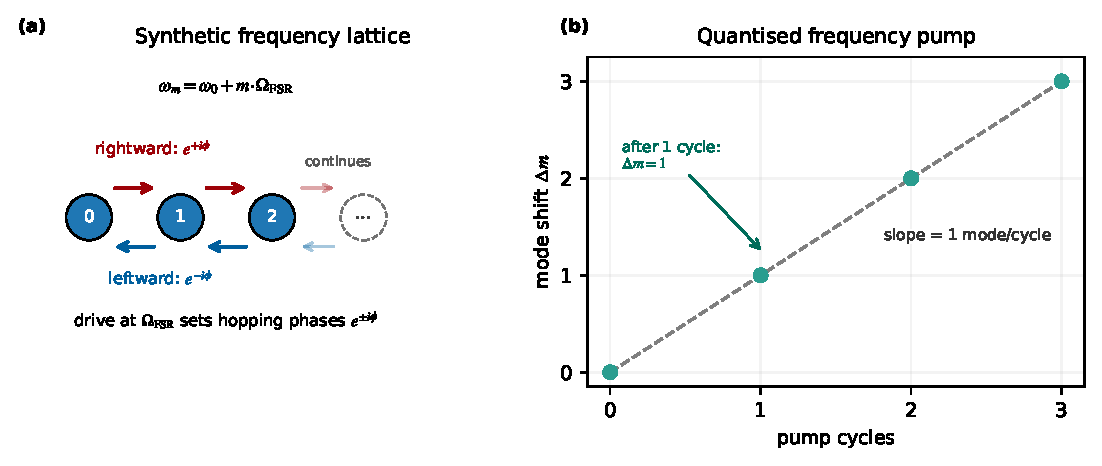
\includegraphics[width=0.92\textwidth]{figures/fig_ch16_synthetic_pump_step199.pdf}
  \caption{Synthetic frequency dimension and topological pumping.
  \textbf{(a)}~Synthetic lattice formed by the frequency modes
  $\omega_m = \omega_0 + m\,\Omega_{\mathrm{FSR}}$ of a ring resonator
  under electro-optic modulation.  Rightward hopping carries a Peierls
  phase $e^{+\ii\phi}$ (red arrows) and leftward hopping carries the
  conjugate $e^{-\ii\phi}$ (blue arrows), realising a gauge field along
  the synthetic axis.  Faded nodes indicate that the lattice continues
  beyond the displayed modes.
  \textbf{(b)}~Quantised topological pump: adiabatic cycling of the
  modulation parameters shifts the mode index by exactly
  $\Delta m = \mathcal{C}_1$ per cycle, where $\mathcal{C}_1$ is the
  first Chern number of the occupied band
  \eqref{eq:ch16-pump-displacement}.  The integer slope of this
  schematic confirms the topological quantisation.}
  \label{fig:ch16-synthetic-pump}
\end{figure}


\subsection{Photonic Thouless pumps}
\label{sec:ch16-photonic-pump}

A photonic Thouless pump can be realised by slowly modulating the
detuning and coupling in a chain of ring resonators.  The modulation
traces a Rice--Mele cycle (Section~\ref{sec:ch14-rice-mele}) in
which the staggered detuning $\Delta(t)$ and dimerisation
$\delta t(t)$ complete a closed orbit around the gap-closing point.

The experimental signature is a quantised shift of the output port:
light injected at one end of the chain emerges shifted by exactly one
unit cell after each pump cycle, regardless of the modulation speed
(as long as it remains adiabatic).  Deviations from quantisation
provide a direct measure of non-adiabatic corrections, which scale
as $(\Omega_{\mathrm{pump}}/\Delta\omega_{\mathrm{gap}})^2$.

Sridhar et~al.\ (2024) demonstrated quantised topological pumping in
a Floquet synthetic dimension using a driven dissipative photonic
molecule \cite{sridhar2024quantized}.  Their system consists of two
coupled microring resonators with periodically modulated coupling,
creating an effective 1D lattice in the Floquet quasi-energy space.
The quantised displacement was measured with a precision of $\pm 3\%$,
limited by residual loss and non-adiabatic corrections.

\subsection{Four-dimensional quantum Hall physics revisited}
\label{sec:ch16-4d-pump}

By extending the pumping to two independent parameters
$(\theta_1,\theta_2)$, one can access four-dimensional topological
physics.  The second Chern number $\Chern_2$, defined on the
four-torus $(k_x,k_y,\theta_1,\theta_2)$, governs the quantised
nonlinear response: a Berry-curvature-induced force proportional
to the product of two pump velocities.

The experimental observation of a $\Chern_2\neq 0$ response in a
2D photonic waveguide array (where two physical coordinates encode
$k_x$ and $\theta_1$, with $\theta_2$ scanned externally) was
reported by Zilberberg et~al.\ (2018).  The measured nonlinear
displacement agreed with the predicted $\Chern_2=1$ to within the
experimental uncertainty of $\sim 8\%$
\cite{ozawa2018topological,price2022roadmap}.

\section{Orbital angular momentum as a synthetic dimension}
\label{sec:ch16-oam-expanded}

\subsection{The OAM ladder}
\label{sec:ch16-oam-ladder}

Photons carry orbital angular momentum (OAM) in units of $\ell\hbar$
per photon, where $\ell$ is the azimuthal index of the Laguerre--Gauss
mode.  In a cylindrically symmetric resonator, modes with different
$\ell$ are degenerate (or nearly so), forming a synthetic lattice
along the OAM axis.

Coupling between adjacent OAM modes ($\ell\to\ell\pm 1$) can be
induced by an element that breaks the cylindrical symmetry---for
example, a tilted mirror, a spatial light modulator, or an
intracavity holographic grating.  The coupling phase depends on the
orientation of the symmetry-breaking element and can be controlled
independently of the coupling strength.

The resulting Hamiltonian is again a tight-binding model on a 1D
lattice (the OAM ladder), and by combining it with a physical
spatial dimension, one obtains a 2D system in which the synthetic
gauge flux per plaquette is determined by the OAM coupling phases
\cite{ozawa2018topological,kim2020recent}.

\subsection{Advantages and limitations}
\label{sec:ch16-oam-advantages}

The OAM synthetic dimension has two key advantages over the frequency
synthetic dimension.  First, the OAM ladder is naturally unbounded
in both directions ($\ell$ ranges from $-\infty$ to $+\infty$),
whereas a frequency comb has a finite bandwidth set by the material
dispersion.  Second, the OAM modes in a resonator can be individually
addressed and measured using spatial light modulators, enabling
site-resolved readout of the synthetic lattice.

The main limitation is that the coupling between OAM modes typically
involves free-space optical elements (spatial light modulators, phase
plates), which are bulky and introduce loss.  Integrated photonic
implementations using ring resonators with asymmetric scatterers are
being developed but have not yet achieved the coupling uniformity
needed for clean topological band structures.

\section{Synthetic Hall ribbons and chiral edge states}
\label{sec:ch16-hall-ribbons}

A particularly elegant application of synthetic dimensions is the
creation of narrow Hall ribbons: quasi-1D systems in which one
dimension is physical and the other (with only a few sites) is
synthetic.  Because the synthetic dimension has a small, controllable
number of sites, the system is effectively a multi-leg ladder rather
than a full 2D lattice.

Mancini et~al.\ (2015) realised a synthetic Hall ribbon using
ultracold fermions in an optical lattice with nuclear spin states
providing the synthetic dimension \cite{mancini2015observation}.
They observed chiral edge currents on opposite legs of the ladder,
a direct manifestation of the topological edge states predicted by
the Hofstadter model on a cylinder.  A complementary experiment by
Stuhl et~al.\ (2015) used bosonic atoms and observed skipping orbits
along the synthetic edges \cite{stuhl2015visualizing}.

In photonics, synthetic Hall ribbons have been proposed using coupled
fibre loops or ring resonator arrays where the synthetic dimension
is provided by the time-bin or frequency degree of freedom.  The
small number of synthetic sites ($N_{\mathrm{syn}}\sim 3$--$5$)
makes these systems particularly amenable to complete experimental
characterisation, including full reconstruction of the edge-state
wave function across both dimensions
\cite{ozawa2018topological,guglielmon2017photonic}.

\section*{Exercises}

\begin{exercise}
  Derive the coupled-mode equation \eqref{eq:ch16-coupled-mode} from
  Maxwell's equations with a time-modulated permittivity
  \eqref{eq:ch16-eps-modulated}, using the rotating-wave approximation.
  State the conditions under which the RWA is valid.
\end{exercise}

\begin{exercise}
  For the 2D Harper--Hofstadter model with flux $\alpha=2\pi/3$, the
  spectrum splits into three subbands.  Using the Diophantine equation,
  determine the Chern number of each subband and verify that the sum
  is zero.
\end{exercise}

\begin{exercise}
  In a ring resonator with free spectral range
  $\Omega_{\mathrm{FSR}}/(2\pi)=10\;\mathrm{GHz}$, modulation depth
  $\eta=0.01$, and carrier frequency $\omega_0/(2\pi)=193\;\mathrm{THz}$,
  compute the effective hopping $\kappa_{\mathrm{eff}}$ and the ratio
  $\kappa_{\mathrm{eff}}/\Omega_{\mathrm{FSR}}$.  Is the tight-binding
  approximation justified?
\end{exercise}

\begin{exercise}
  The second Chern number $\Chern_2$ of a 4D quantum Hall state
  determines the quantised nonlinear Hall response.  If the system has
  $\Chern_2=1$ and two of the four dimensions are synthetic (frequency
  modes), describe how the nonlinear response manifests as a measurable
  photonic observable.
\end{exercise}

\begin{exercise}
  Design a synthetic-dimension experiment using OAM modes of a ring
  resonator.  Specify the coupling mechanism, the expected bandwidth
  of the synthetic dimension (number of usable OAM modes), and the
  modulation phase that creates a gauge flux of $\alpha=\pi/2$ per
  plaquette.
\end{exercise}

\begin{exercise}
  Compare the advantages and limitations of synthetic dimensions versus
  physical spatial dimensions for realising topological photonic phases.
  In what situations would each approach be preferred?
\end{exercise}
